\documentclass{standalone}
\usepackage{tikz}
\usepackage{xcolor, soul}
\usetikzlibrary{matrix, positioning}
\newcommand{\dT}[0]{\setulcolor{red}{\ul{T}}}
\newcommand{\dG}[0]{\setulcolor{green}{\ul{G}}}
\newcommand{\dC}[0]{\setulcolor{yellow}{\ul{C}}}
\newcommand{\dA}[0]{\setulcolor{blue}{\ul{A}}}
\begin{document}
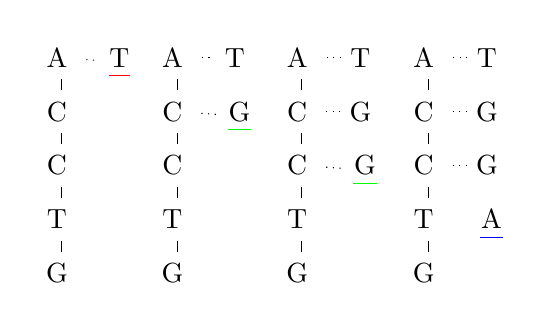
\begin{tikzpicture}
  \matrix (m) [matrix of math nodes, align=center, row sep=0.2em, column sep=0.5em, minimum width=1em, minimum height=1.5em]{
A & \dT  &A & T   &A & T   &A & T   \\
C &      &C & \dG &C & G   &C & G   \\
C &      &C &     &C & \dG &C & G   \\
T &      &T &     &T &     &T & \dA \\
G &      &G &     &G &     &G &     \\
};
\draw (m-1-1) -- (m-2-1) -- (m-3-1) -- (m-4-1) -- (m-5-1);
\draw[dotted] (m-1-1) -- (m-1-2);
\draw (m-1-3) -- (m-2-3) -- (m-3-3) -- (m-4-3) -- (m-5-3);
\draw[dotted] (m-1-3) -- (m-1-4);
\draw[dotted] (m-2-3) -- (m-2-4);
\draw (m-1-5) -- (m-2-5) -- (m-3-5) -- (m-4-5) -- (m-5-5);
\draw[dotted] (m-1-5) -- (m-1-6);
\draw[dotted] (m-2-5) -- (m-2-6);
\draw[dotted] (m-3-5) -- (m-3-6);
\draw (m-1-7) -- (m-2-7) -- (m-3-7) -- (m-4-7) -- (m-5-7);
\draw[dotted] (m-1-7) -- (m-1-8);
\draw[dotted] (m-2-7) -- (m-2-8);
\draw[dotted] (m-3-7) -- (m-3-8);
\end{tikzpicture}
\end{document}

%%% Local Variables:
%%% mode: latex
%%% TeX-master: t
%%% End:
